\documentclass[12pt,letterpaper]{article}
\usepackage{graphicx,textcomp}
\usepackage{natbib}
\usepackage{setspace}
\usepackage{fullpage}
\usepackage{color}
\usepackage[reqno]{amsmath}
\usepackage{amsthm}
\usepackage{fancyvrb}
\usepackage{amssymb,enumerate}
\usepackage[all]{xy}
\usepackage{endnotes}
\usepackage{lscape}
\newtheorem{com}{Comment}
\usepackage{float}
\usepackage{hyperref}
\newtheorem{lem} {Lemma}
\newtheorem{prop}{Proposition}
\newtheorem{thm}{Theorem}
\newtheorem{defn}{Definition}
\newtheorem{cor}{Corollary}
\newtheorem{obs}{Observation}
\usepackage[compact]{titlesec}
\usepackage{dcolumn}
\usepackage{tikz}
\usetikzlibrary{arrows}
\usepackage{multirow}
\usepackage{xcolor}
\newcolumntype{.}{D{.}{.}{-1}}
\newcolumntype{d}[1]{D{.}{.}{#1}}
\definecolor{light-gray}{gray}{0.65}
\usepackage{url}
\usepackage{listings}
\usepackage{color}

\definecolor{codegreen}{rgb}{0,0.6,0}
\definecolor{codegray}{rgb}{0.5,0.5,0.5}
\definecolor{codepurple}{rgb}{0.58,0,0.82}
\definecolor{backcolour}{rgb}{0.95,0.95,0.92}

\lstdefinestyle{mystyle}{
	backgroundcolor=\color{backcolour},   
	commentstyle=\color{codegreen},
	keywordstyle=\color{magenta},
	numberstyle=\tiny\color{codegray},
	stringstyle=\color{codepurple},
	basicstyle=\footnotesize,
	breakatwhitespace=false,         
	breaklines=true,                 
	captionpos=b,                    
	keepspaces=true,                 
	numbers=left,                    
	numbersep=5pt,                  
	showspaces=false,                
	showstringspaces=false,
	showtabs=false,                  
	tabsize=2
}
\lstset{style=mystyle}
\newcommand{\Sref}[1]{Section~\ref{#1}}
\newtheorem{hyp}{Hypothesis}

\title{Problem Set 1}
<<<<<<< HEAD
\date{Due: October 3, 2021}
\author{Conor Twomey Student No. 22996168
	 Applied Stats/Quant Methods 1}
=======
\date{Due: October 3, 2022}
\author{Applied Stats/Quant Methods 1}
>>>>>>> af2a91eef73f36234332980a3a4c406b0f477d9e

\begin{document}
	\maketitle
	
	\section*{Instructions}
	\begin{itemize}
		\item Please show your work! You may lose points by simply writing in the answer. If the problem requires you to execute commands in \texttt{R}, please include the code you used to get your answers. Please also include the \texttt{.R} file that contains your code. If you are not sure if work needs to be shown for a particular problem, please ask.
		\item Your homework should be submitted electronically on GitHub.
		\item This problem set is due before class on Monday October 3, 2022. No late assignments will be accepted.
		\item Total available points for this homework is 80.
	\end{itemize}
	
	\vspace{1cm}
<<<<<<< HEAD
	\section*{Question 1 (50 points): Education}
	
	A school counselor was curious about the average of IQ of the students in her school and took a random sample of 25 students' IQ scores. The following is the data set:\\
	\vspace{.5cm}
	
	\vspace{1cm}
	
	\begin{enumerate}
		\item Find a 90\% confidence interval for the average student IQ in the school.\\
	\end{enumerate}

\lstinputlisting[language=R, firstline=40, lastline=62]{PS01.R}

\begin{verbatim}
	    Lower :  94.13283  Upper : 102.7472
\end{verbatim}

\lstinputlisting[language=R, firstline=63, lastline=64\\\\]{PS01.R}
 \begin{verbatim}
 2.618575
 \end{verbatim}

\lstinputlisting[language=R, firstline=66, lastline=66\\\\]{PS01.R}
 \begin{verbatim}
1.710882
\end{verbatim}

\lstinputlisting[language=R, firstline=68, lastline=68\\\\]{PS01.R}
\begin{verbatim}
	93.95993
\end{verbatim}

\lstinputlisting[language=R, firstline=70, lastline=70\\\\]{PS01.R}
\begin{verbatim}
102.9201
\end{verbatim}
		
	\begin{enumerate}
		\item Next, the school counselor was curious  whether  the average student IQ in her school is higher than the average IQ score (100) among all the schools in the country.\\ 
		
		\noindent Using the same sample, conduct the appropriate hypothesis test with $\alpha=0.05$.
	\end{enumerate}

\begin{verbatim}
	Hypothesis testing
	
	Step 1 : I assuming that this is a normal distribution
	
	Step 2: The null hypothesis is that ybar is less than or equal to 100
				The alternative hypothesis is that ybar is greater than 100
				
	Step 3: Calculating the t-statistic 
\end{verbatim}
\lstinputlisting[language=R, firstline=87, lastline=88\\\\]{PS01.R}
	\begin{verbatim}
-0.5957439
	\end{verbatim}

\lstinputlisting[language=R, firstline=90, lastline=95\\\\]{PS01.R}
	\begin{verbatim}
One Sample t-testdata:  yt = -0.59574, df = 24, p-value = 0.7215
Alternative hypothesis: true
Mean is greater than 100
95 percent confidence interval: 93.95993      
Infsample estimates:mean of x     98.44 
\end{verbatim}


	
	\newpage
	
	\section*{Question 2 (50 points): Political Economy}
	
	\noindent Researchers are curious about what affects the amount of money communities spend on addressing homelessness. The following variables constitute our data set about social welfare expenditures in the USA. \\

	
	
	\begin{tabular}{r|l}
		\texttt{State} &\emph{50 states in US} \\
		\texttt{Y} & \emph{per capita expenditure on shelters/housing assistance in state}\\
		\texttt{X1} &\emph{per capita personal income in state} \\
		\texttt{X2} &  \emph{Number of residents per 100,000 that are "financially insecure" in state}\\
		\texttt{X3} &  \emph{Number of people per thousand residing in urban areas in state} \\
		\texttt{Region} &  \emph{1=Northeast, 2= North Central, 3= South, 4=West} \\
	\end{tabular}
	
	\vspace{.5cm}
	\noindent Explore the \texttt{expenditure} data set and import data into \texttt{R}.
	\vspace{.5cm}
	\lstinputlisting[language=R, firstline=54, lastline=54]{PS01.R}  
	\vspace{.5cm}
	\begin{itemize}
		\item
		Please plot the relationships among \emph{Y}, \emph{X1}, \emph{X2}, and \emph{X3}? What are the correlations among them (you just need to describe the graph and the relationships among them)?
		\end{itemize}
		
		\begin{figure}[h!]
			\centering
			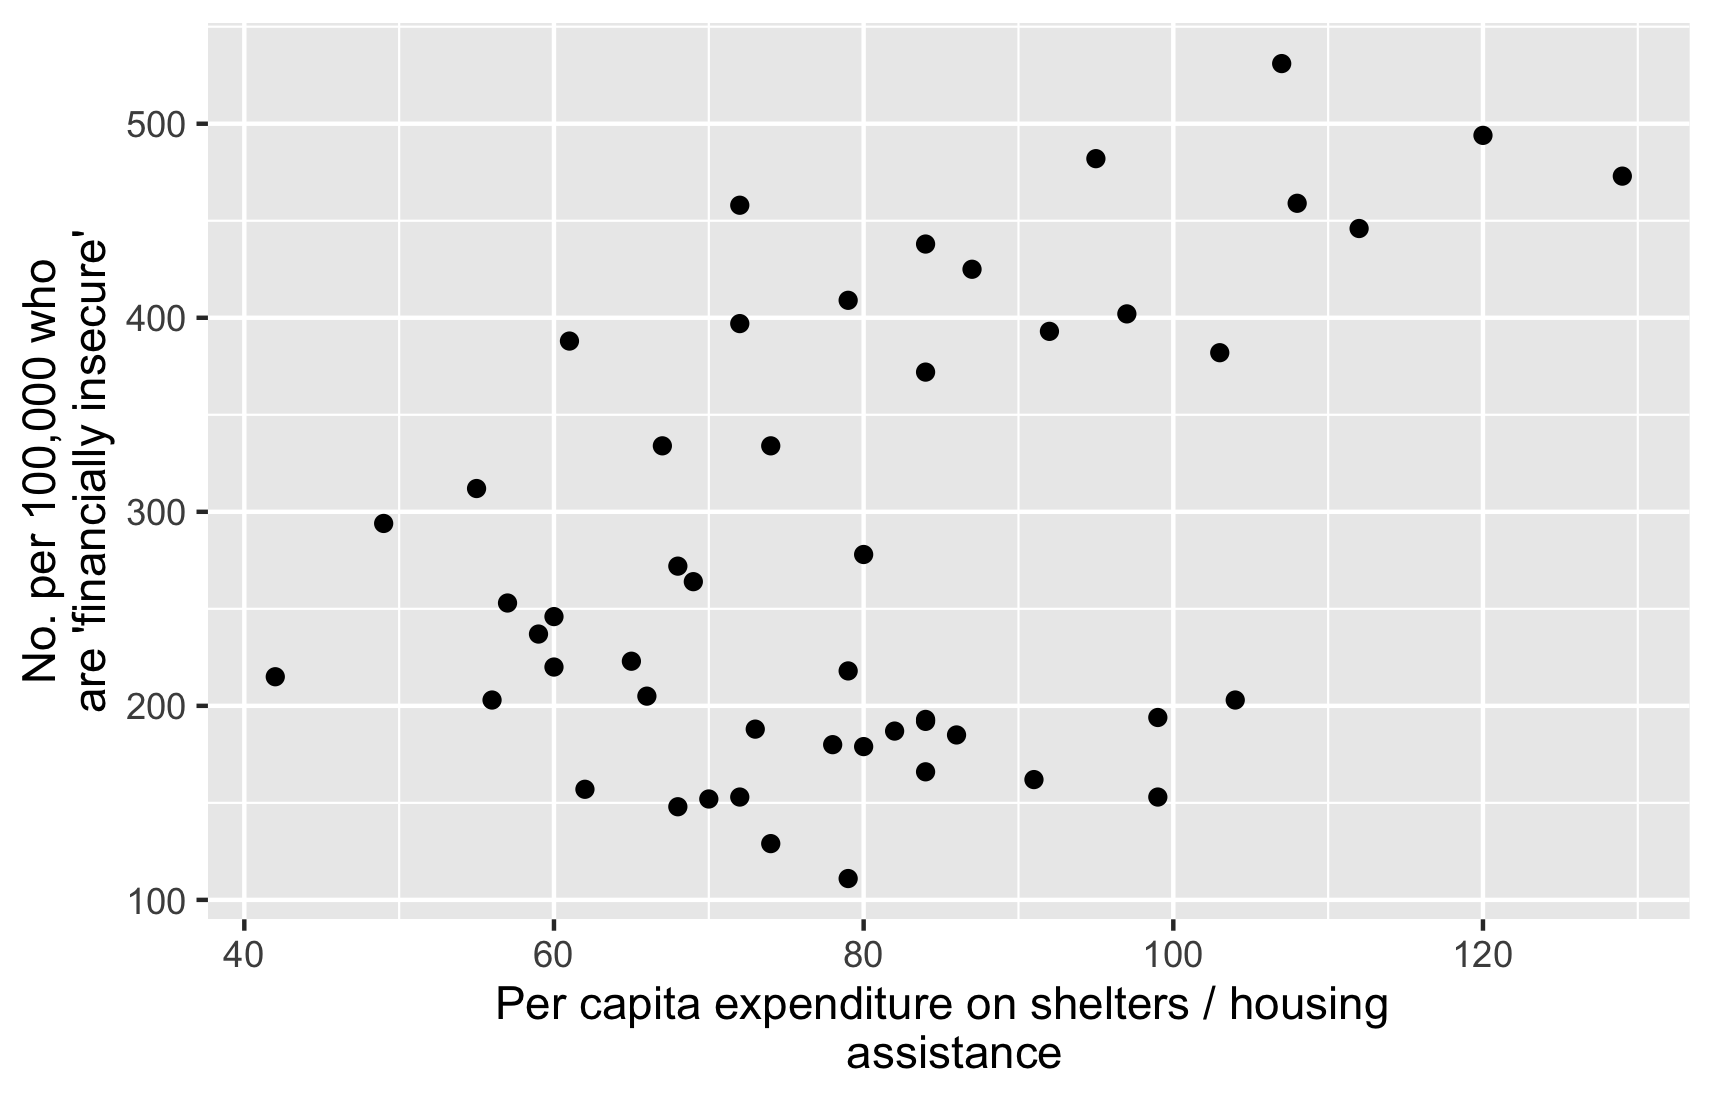
\includegraphics[width=0.7\linewidth]{../yx1}
			\caption{Y and X1 plot\\}
			\label{fig:yx1}
		\end{figure}
	\begin{verbatim}
The relationship between these variables is broadly linear however there are a 
few outliers with a cluster at the bottom of the plot
	\end{verbatim}
		
		\begin{figure}[h!]
		\centering
		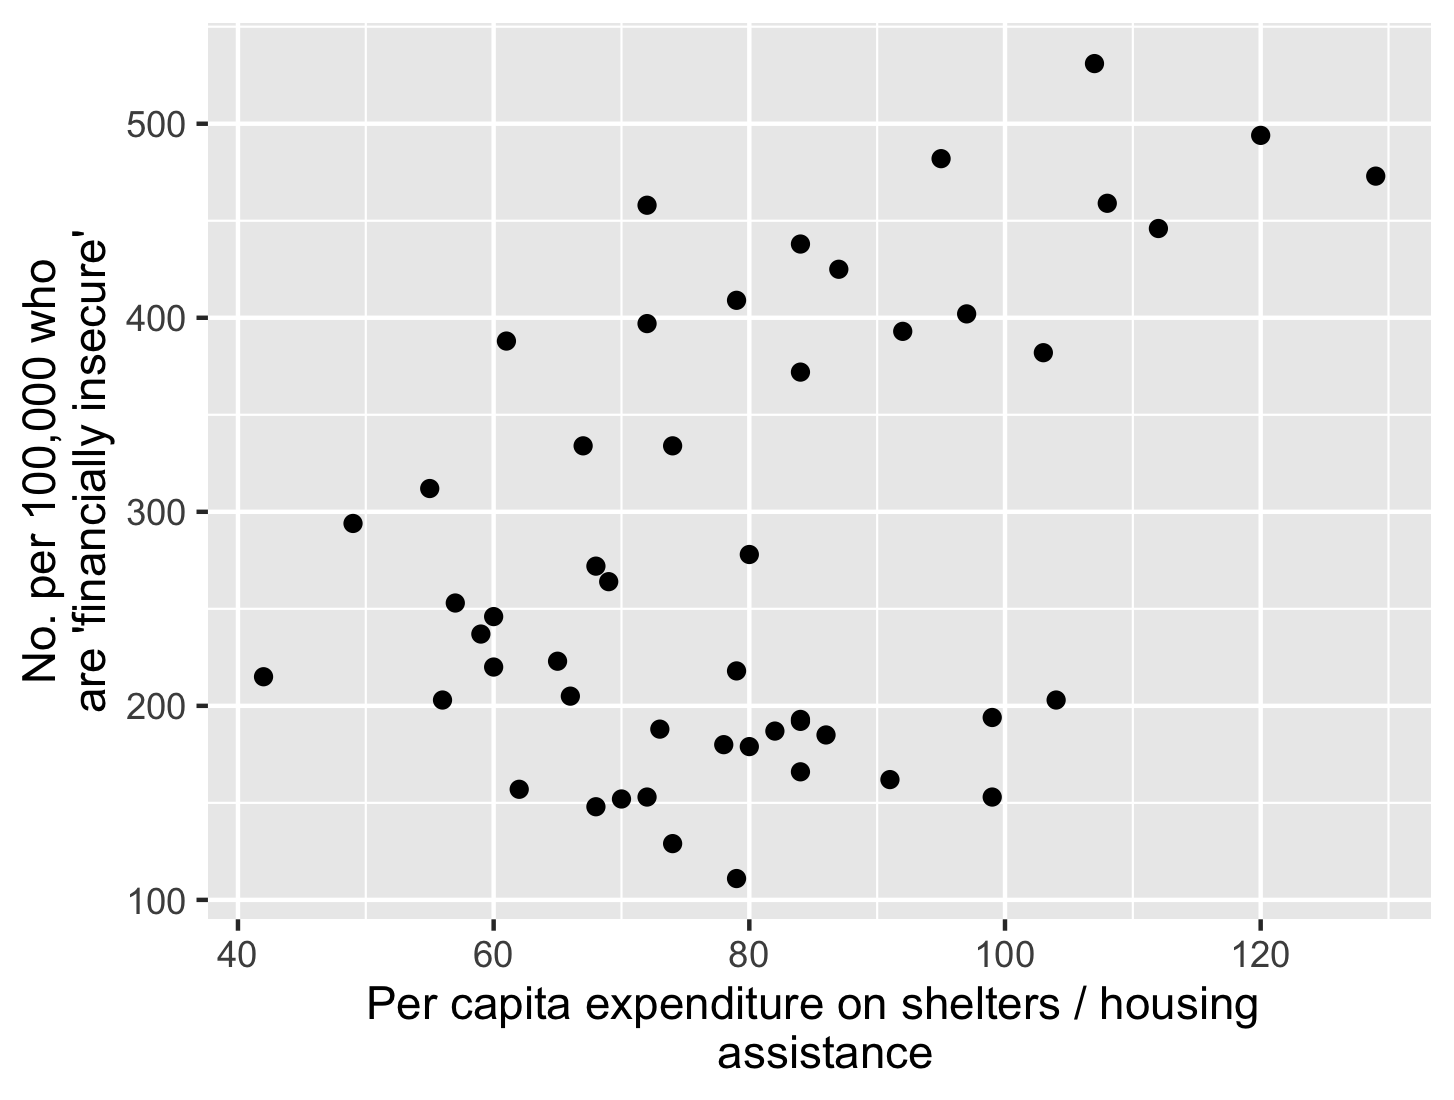
\includegraphics[width=0.7\linewidth]{../plot2}
		\caption{Y and X2 plot}
		\label{fig:Y and X2}
		\end{figure}
	\begin{verbatim}
The relationship between these variables is broadly linear however there are a few outliers 
\end{verbatim}

\begin{figure}[H]
	\centering
	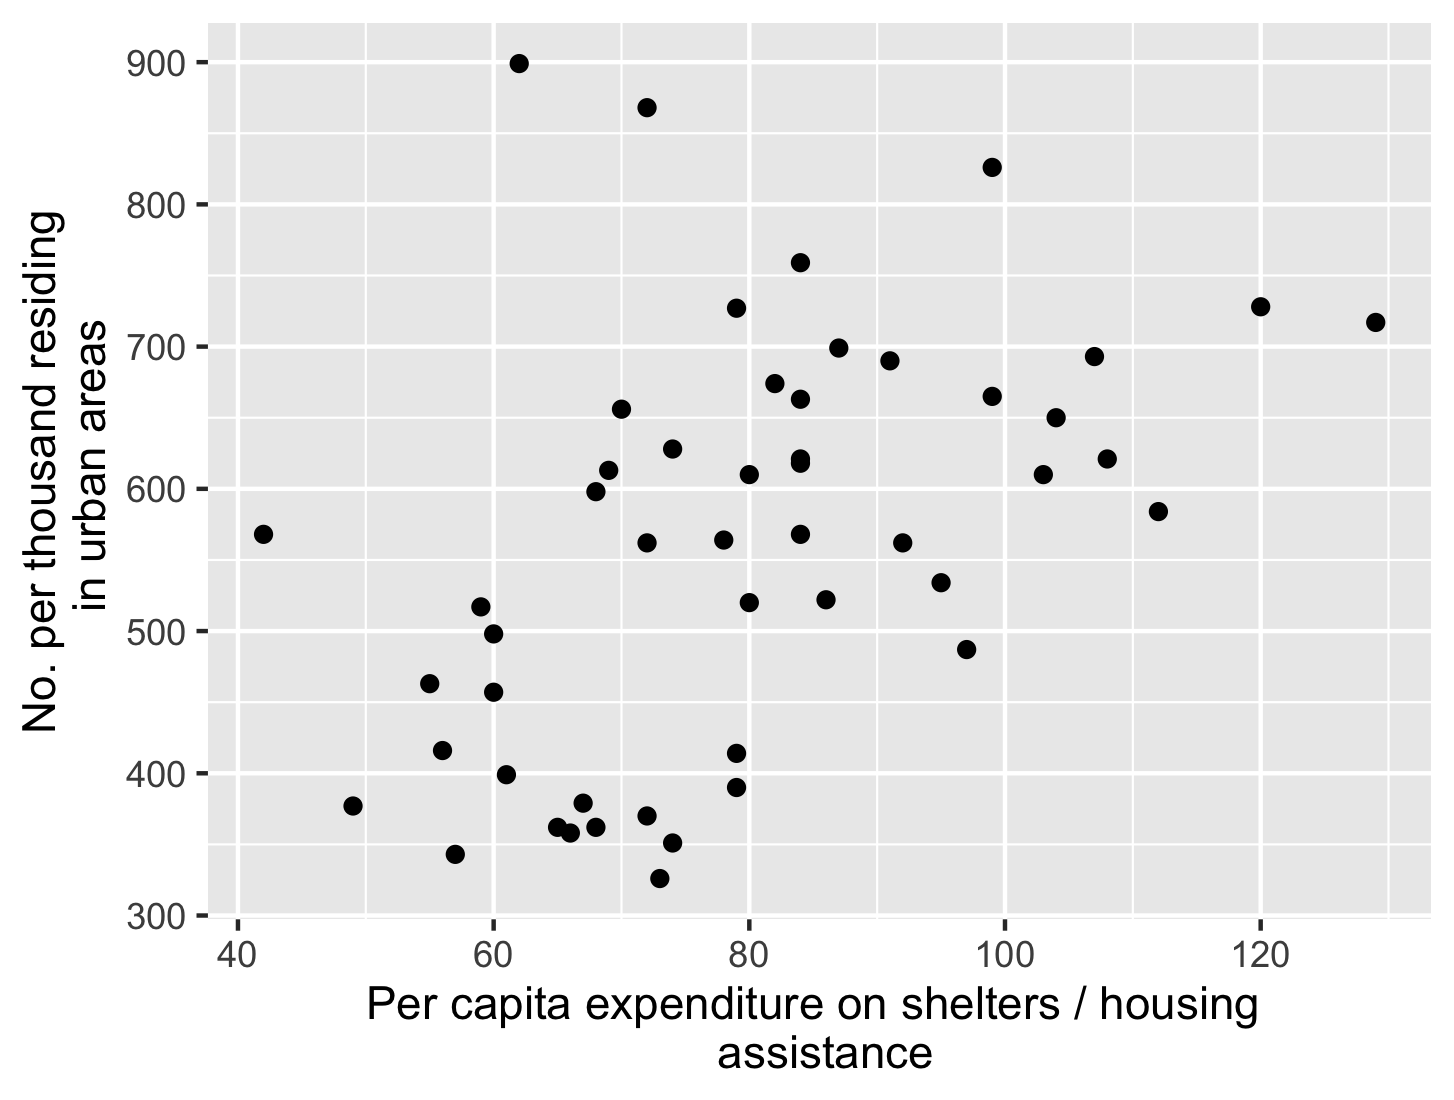
\includegraphics[width=0.7\linewidth]{../plot3}
	\caption{}
	\label{fig:plot3}
\end{figure}


	\begin{verbatim}
	There is a somewhat linear relationship between these variables
\end{verbatim}
\vspace{.5cm}

	\begin{figure}[H]
	\centering
	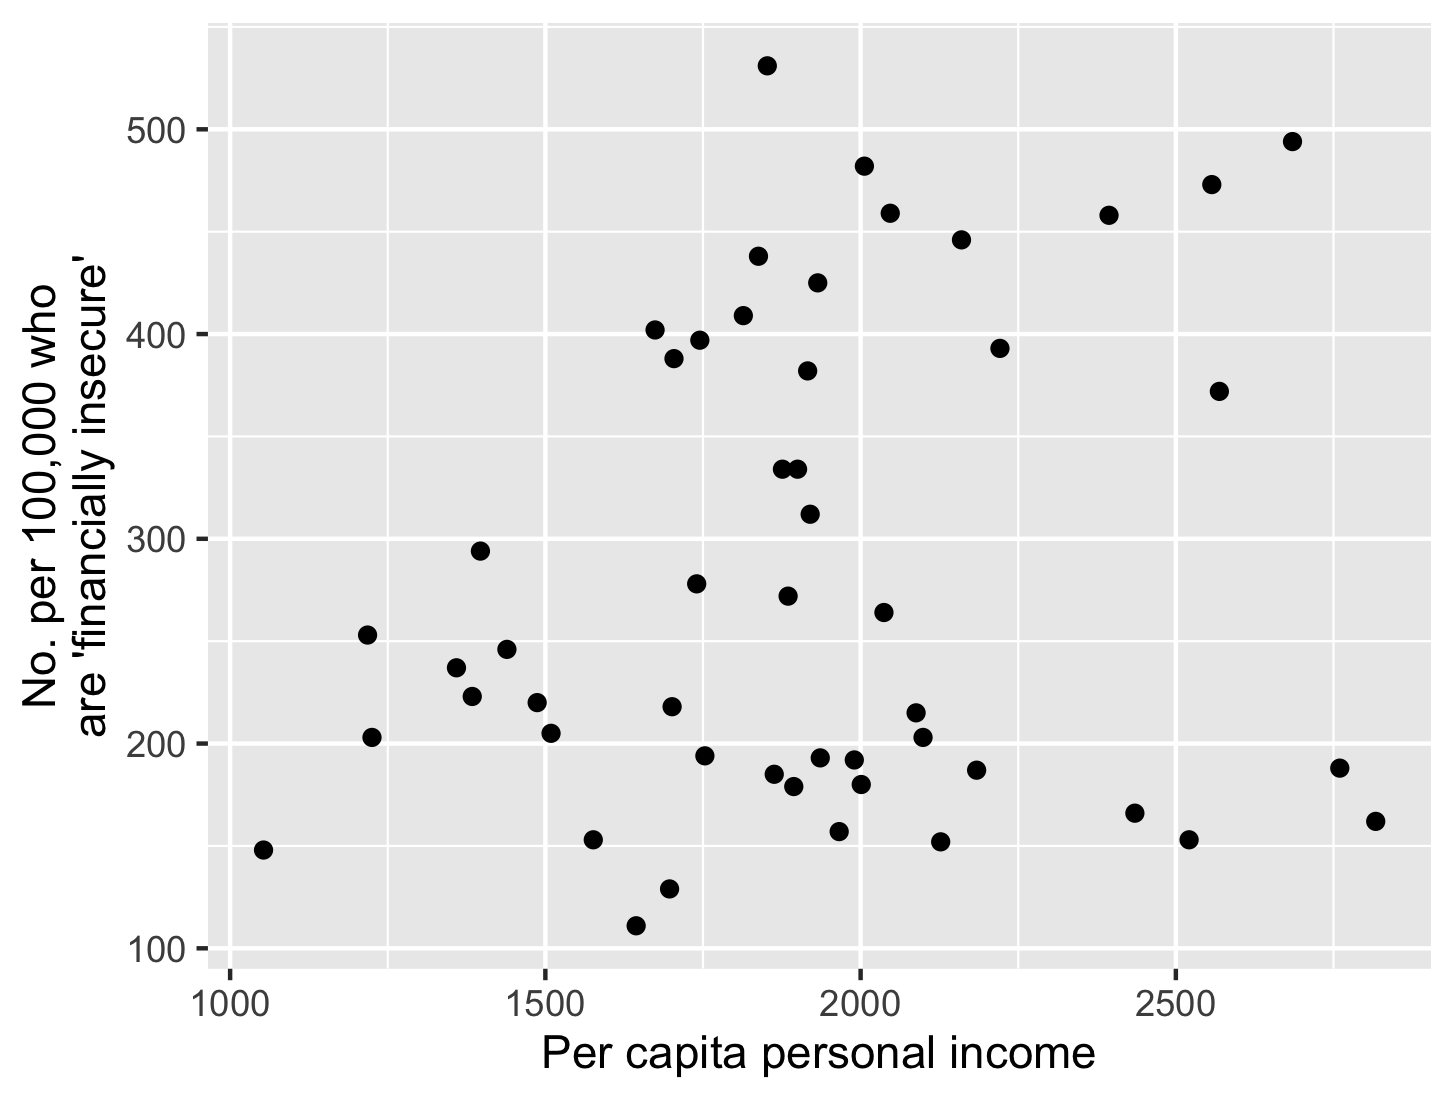
\includegraphics[width=0.7\linewidth]{../plot4}
	\caption{X1 and X2 plot}
	\label{fig:plot4}
	\end{figure}

	\begin{verbatim}
There is not a linear relationship between these variables
\end{verbatim}

\begin{figure}[H]
	\centering
	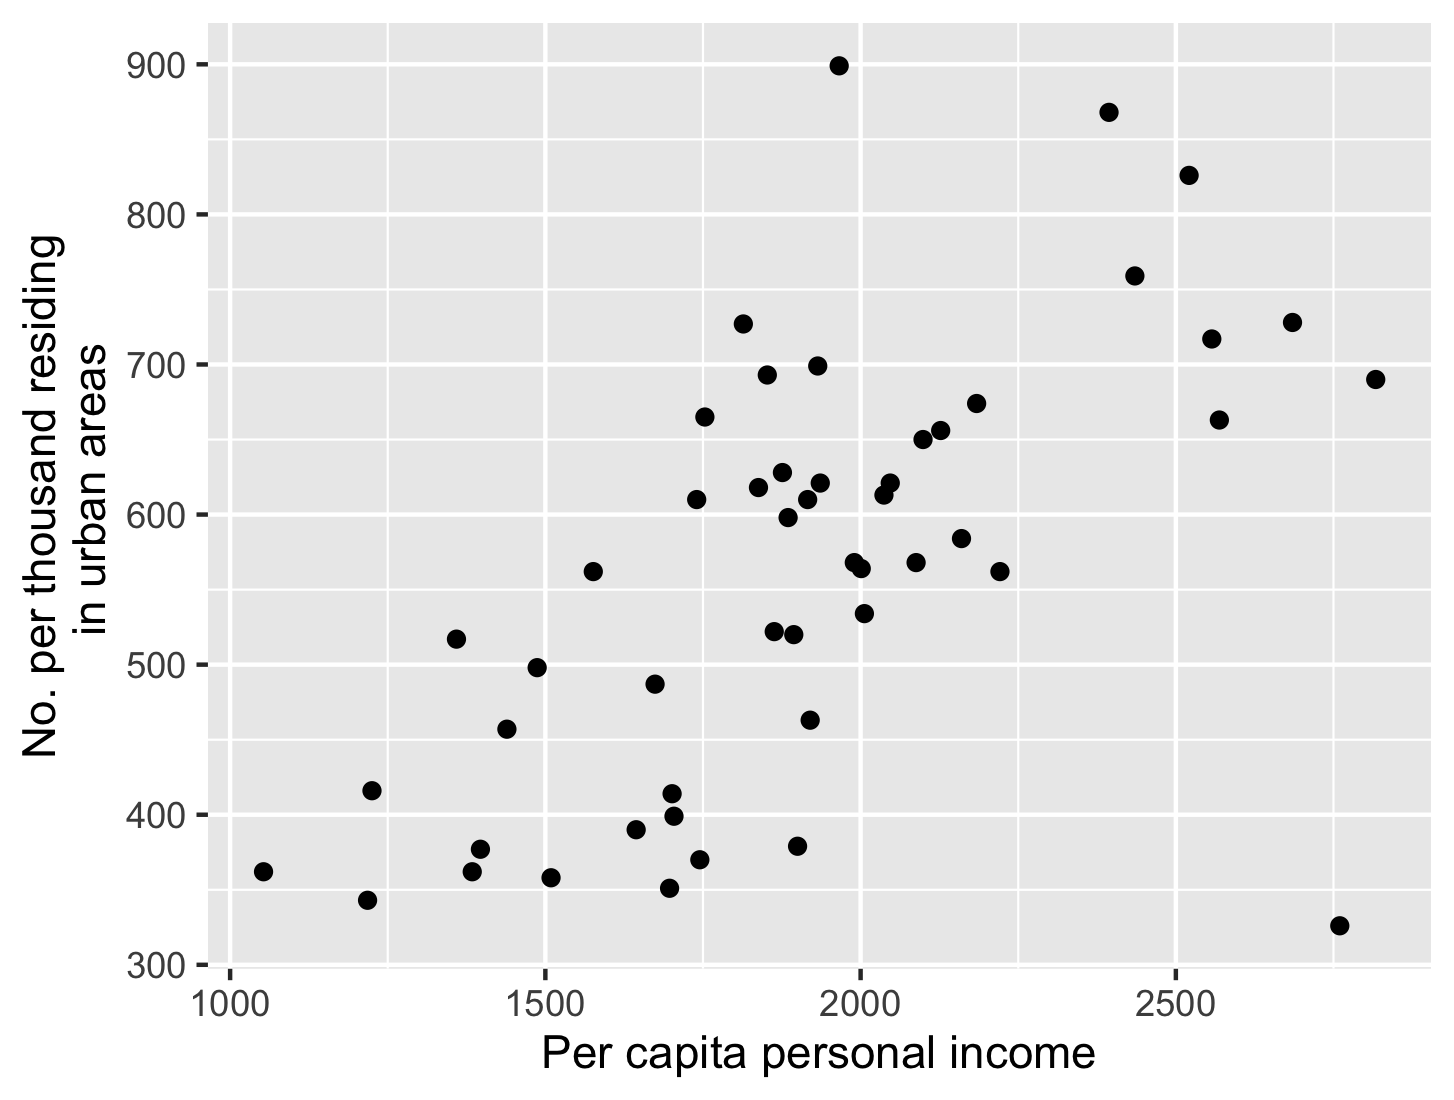
\includegraphics[width=0.7\linewidth]{../plot5}
	\caption{}
	\label{fig:plot5}
\end{figure}

	\begin{verbatim}
	There is a linear relationship between these variables
\end{verbatim}


\begin{figure}[H]
	\centering
	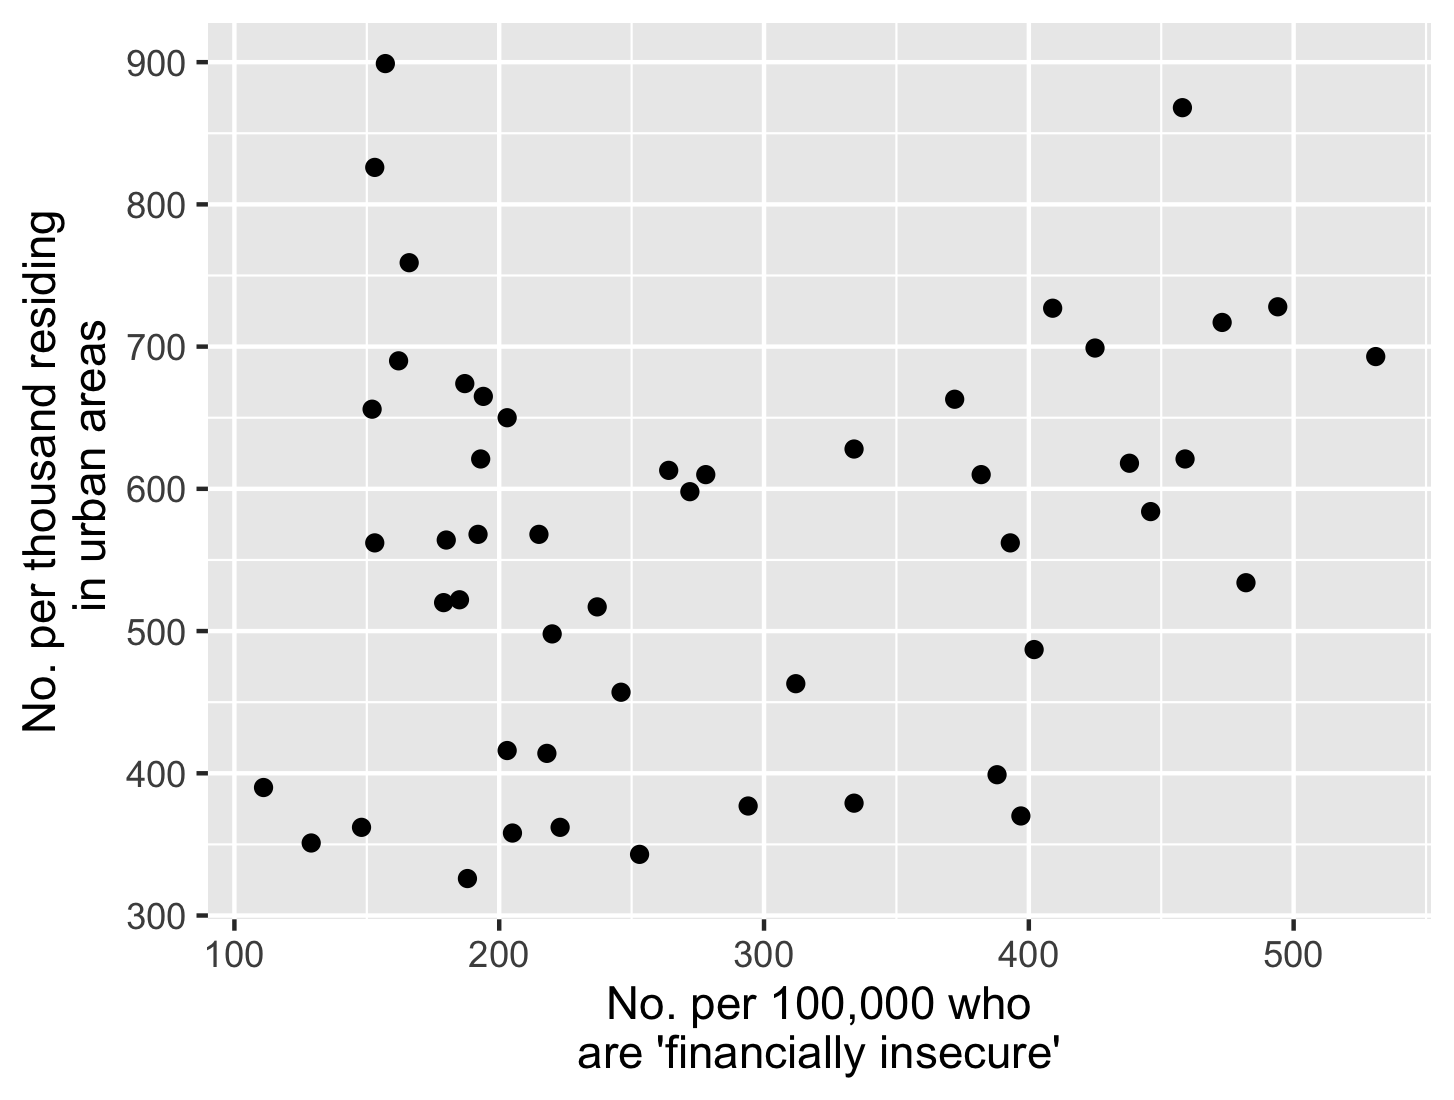
\includegraphics[width=0.7\linewidth]{../plot6}
	\caption{}
	\label{fig:plot6}
\end{figure}

	\begin{verbatim}
	There is no relationship between these variables 
\end{verbatim}
	\vspace{1cm}



		\begin{itemize}
			\item 	Please plot the relationship between \emph{Y} and \emph{Region}? On average, which region has the highest per capita expenditure on housing assistance?
		\end{itemize}

	
		\begin{figure}[H]
			\centering
			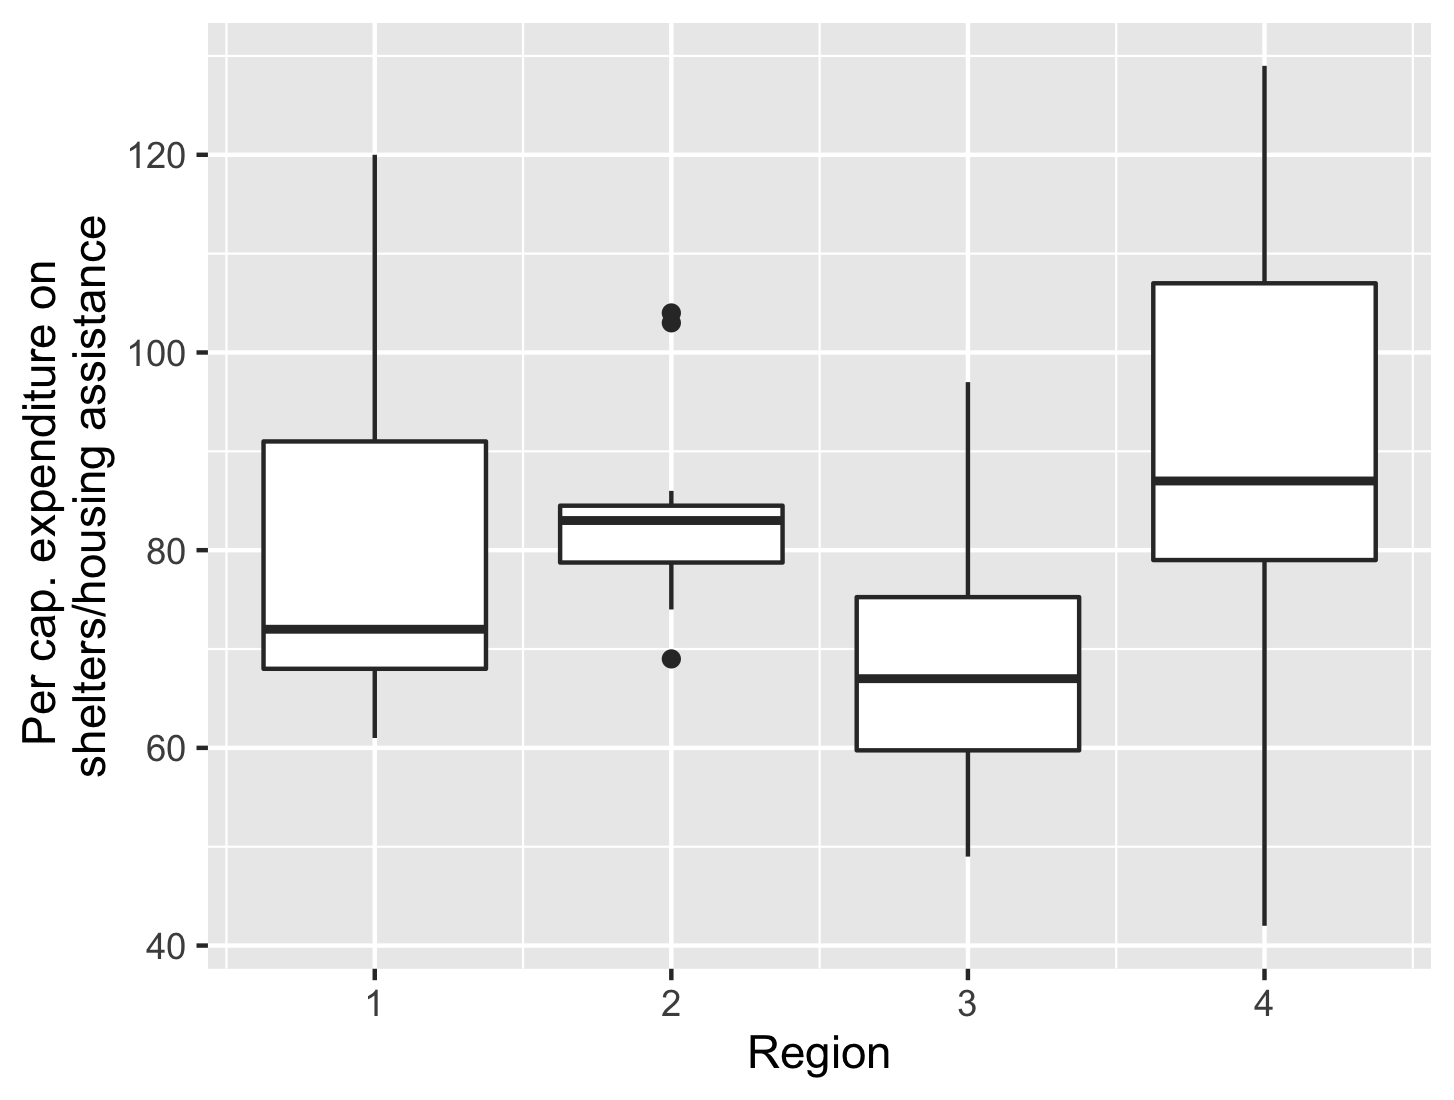
\includegraphics[width=0.7\linewidth]{../plot7}
			\caption{}
			\label{fig:plot7}
		\end{figure}

	\begin{verbatim}
Region 4 (West) spends the most on average per capita on shelters/ housing assistance
\end{verbatim}
	\vspace{10cm}

		\begin{itemize}
			\item 	Please plot the relationship between \emph{Y} and \emph{X1}? Describe this graph and the relationship. Reproduce the above graph including one more variable \emph{Region} and display different regions with different types of symbols and colors.
		\end{itemize}
	

\begin{figure}[H]
	\centering
	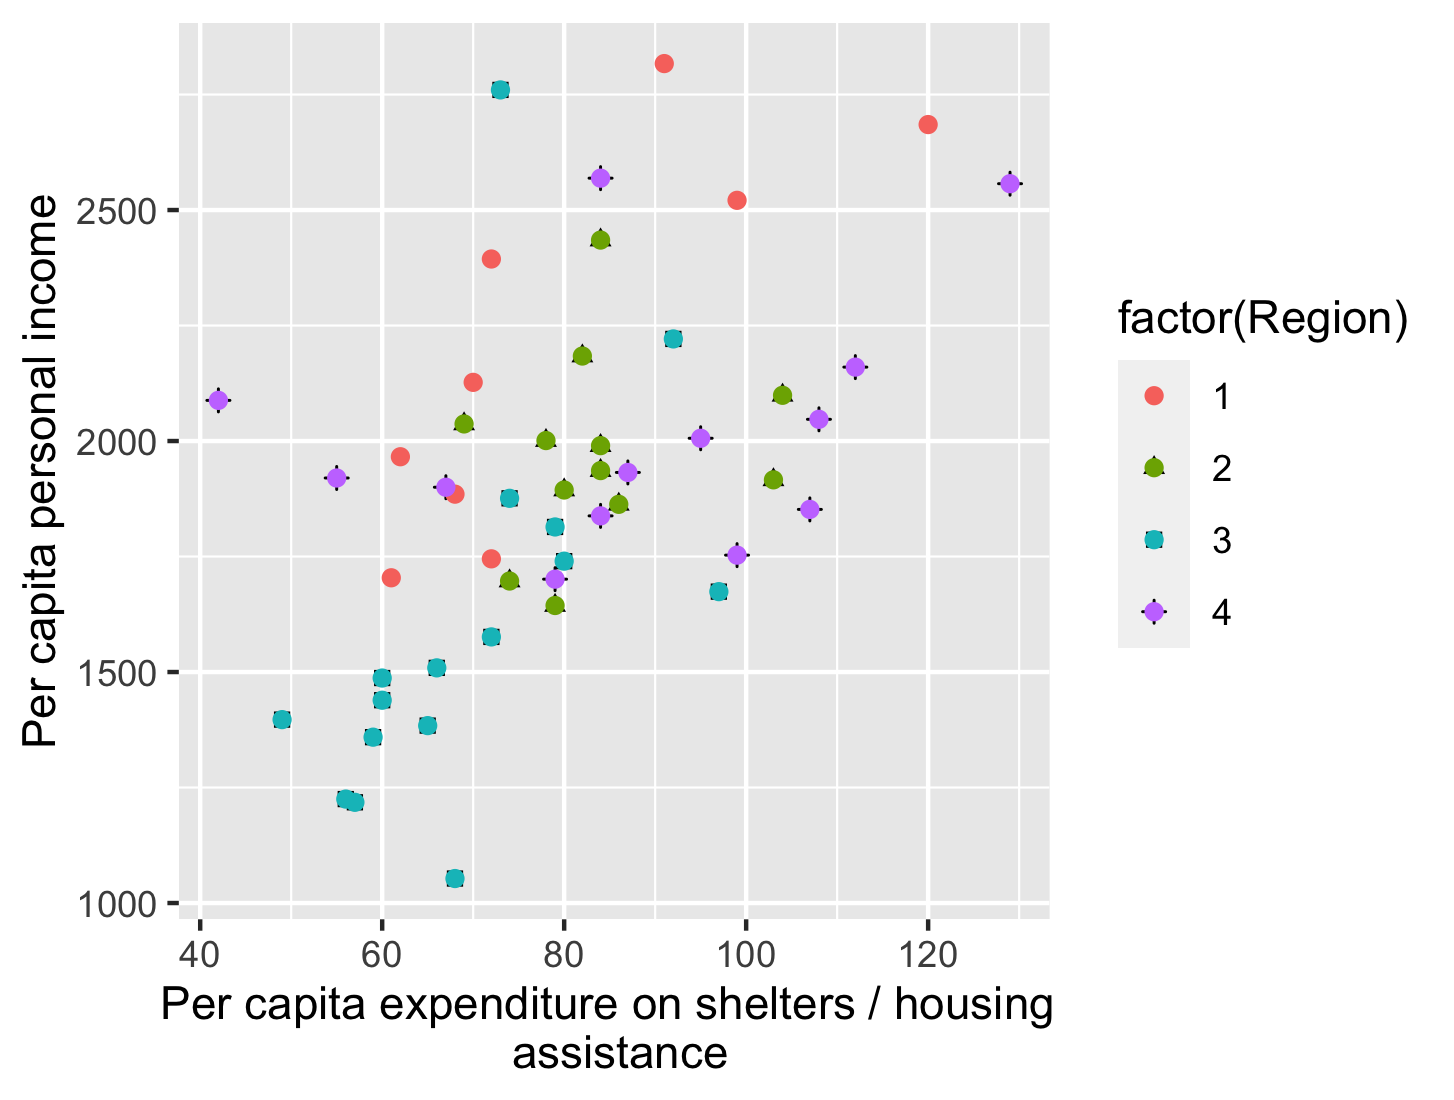
\includegraphics[width=0.7\linewidth]{../plot8}
	\caption{Y and X1 plot with Region variable}
	\label{fig:plot8}
\end{figure}

=======
	\section*{Question 1 (40 points): Education}

A school counselor was curious about the average of IQ of the students in her school and took a random sample of 25 students' IQ scores. The following is the data set:\\
\vspace{.5cm}

\lstinputlisting[language=R, firstline=40, lastline=40]{PS01.R}  

\vspace{1cm}

\begin{enumerate}
	\item Find a 90\% confidence interval for the average student IQ in the school.\\
>>>>>>> af2a91eef73f36234332980a3a4c406b0f477d9e
	
	\item Next, the school counselor was curious  whether  the average student IQ in her school is higher than the average IQ score (100) among all the schools in the country.\\ 
	
	\noindent Using the same sample, conduct the appropriate hypothesis test with $\alpha=0.05$.
\end{enumerate}

\newpage

	\section*{Question 2 (40 points): Political Economy}

\noindent Researchers are curious about what affects the amount of money communities spend on addressing homelessness. The following variables constitute our data set about social welfare expenditures in the USA. \\
\vspace{.5cm}


\begin{tabular}{r|l}
	\texttt{State} &\emph{50 states in US} \\
	\texttt{Y} & \emph{per capita expenditure on shelters/housing assistance in state}\\
	\texttt{X1} &\emph{per capita personal income in state} \\
	\texttt{X2} &  \emph{Number of residents per 100,000 that are "financially insecure" in state}\\
	\texttt{X3} &  \emph{Number of people per thousand residing in urban areas in state} \\
	\texttt{Region} &  \emph{1=Northeast, 2= North Central, 3= South, 4=West} \\
\end{tabular}

\vspace{.5cm}
\noindent Explore the \texttt{expenditure} data set and import data into \texttt{R}.
\vspace{.5cm}
\lstinputlisting[language=R, firstline=54, lastline=54]{PS01.R}  
\vspace{.5cm}
\begin{itemize}

\item
Please plot the relationships among \emph{Y}, \emph{X1}, \emph{X2}, and \emph{X3}? What are the correlations among them (you just need to describe the graph and the relationships among them)?
\vspace{.5cm}
\item
Please plot the relationship between \emph{Y} and \emph{Region}? On average, which region has the highest per capita expenditure on housing assistance?
\vspace{.5cm}
\item
Please plot the relationship between \emph{Y} and \emph{X1}? Describe this graph and the relationship. Reproduce the above graph including one more variable \emph{Region} and display different regions with different types of symbols and colors.
\end{itemize}


\end{document}
